\section{Evaluation}

Our experiment with \CoBBl~aims to answer the following questions:
\begin{enumerate}
  \item How does \CoBBl~perform compare to the state-of-the-art direct-translator on (a) compiler time, (b) prover time (c) verifier time, and (d) proof size?\label{q:performance-dt}
  \item How does \CoBBl~perform compare to the state-of-the-art virtual machine on the four metrics in question \ref{q:performance-dt}?\label{q:performance-vm}
  \item How does smaller circuit size produced by \CoBBl's block-based abstractions affect performance, in comparison to the overhead introduced by the additional program states?\label{q:tradeoff}
\end{enumerate}

We choose CirC~\cite{ozdemir20circ} as the baseline for state-of-the-art direct translator, and Jolt~\cite{arun23jolt} as the baseline for virtual machine. \red{[XXX: Need justification? Where to mention that Jolt has an industrial-level budget?]} We conduct the experiments on implementations of \CoBBl, CirC and Jolt across 7 benchmarks.

\subsection{Implementation}
\red{[XXX: Will there be a separate implementation section? Some details might be interesting to go through]} We base the frontend compiler of \CoBBl~on existing infrastructure of CirC, our direct translator baseline, as CirC contains most underlying functionalities required by \CoBBl~(in particular, conversion of high-level languages to constraints). On top of CirC, we implement \CoBBl's frontend through 7000 lines of Rust code: dividing a program in to segments, performing all optimizations on each segment, and repackaging each segment as individual programs recognizable by CirC's direct translator. We apply minimal modification to CirC's internal codebase to ensure fairness of comparison.

The backend proof system for \CoBBl~is a custom variant of Spartan~\cite{setty19spartan}, the same proof system used by our two baselines. We modify Spartan through 7000 lines of Rust code to support parallel execution of all program segments, but leave most internal logic untouched.

\subsection{Baselines and Benchmarks}
\paragraph{CirC} We modify CirC to support branching statements to align with our benchmarks, using exclusively existing functionalities. Apart from updates to the parser and input format, everything else stays the same as the original codebase~\cite{circ_codebase}.

\paragraph{Jolt} Our Jolt evaluation uses the released codebase~\cite{jolt_codebase}.

\paragraph{Benchmarks} Figure \ref{fig:benchmark_overview} lists our benchmarks. We implement each benchmark in two programming languages: the Zokrates version is used by \CoBBl~and CirC, while the Rust version is used by Jolt, compiled with release mode (\code{--release}). The two versions of each benchmark are identical up to grammatical differences. Since CirC generally performs far worse than Jolt, we choose a different set of parameters when comparing \CoBBl~against CirC than Jolt. All benchmarks except for Poseidon are computed exclusively using 32-bit registers -- the native instruction set for Jolt -- to ensure Jolt's maximum efficiency. We explore the special scenario introduced by Poseidon later in the section.

\paragraph{Special Benchmark} To answer question \ref{q:tradeoff}, we conduct a separate test on the Find Min benchmark, recording detailed performance of CirC and \CoBBl~for array length ranging from 200 to 1600.

\begin{table}[t]
  \begin{tabular}{l l l}
    \centering
    \textbf{Benchmarks} & \textbf{Parameters} & \textbf{Type} \\
    \hline \\
    \makecell[l]{Min value in an array \\ (Find Min)} & \makecell[l]{\emph{v. CirC}: len = 1200 \\ \emph{v. Jolt}: len = 1200} & 32-bit \\
    \vspace{2\baselineskip}\\
    \makecell[l]{Matrix Multiplication \\ (Mat Mult)} & \makecell[l]{\emph{v. CirC}: size = 8x8 \\ \emph{v. Jolt}: size = 16x16} & 32-bit \\
    \vspace{2\baselineskip}\\
    \makecell[l]{KMP pattern match \\ (Pat Match)} & \makecell[l]{\emph{v. CirC}: pat / txt = 48 / 480 \\ \emph{v. Jolt}: pat / txt = 48 / 480} & 32-bit \\
    \vspace{2\baselineskip}\\
    \makecell[l]{Largest common subsequence \\ (LCS)} & \makecell[l]{\emph{v. CirC}: len = 5 \\ \emph{v. Jolt}: len = 30} & 32-bit \\
    \vspace{2\baselineskip}\\
    \makecell[l]{RLE encode + decode \\ (RLE)} & \makecell[l]{\emph{v. CirC}: len = 20 \\ \emph{v. Jolt}: len = 60} & 32-bit \\
    \vspace{2\baselineskip}\\
    \makecell[l]{Sha-256 Hashing \\ (Sha256)} & \makecell[l]{\emph{v. CirC}: len = 1 \\ \emph{v. Jolt}: len = 6} & 32-bit \\
    \vspace{2\baselineskip}\\
    \makecell[l]{Poseidon Hashing \\ (Poseidon)} & \makecell[l]{\emph{v. CirC}: len = 3 \\ \emph{v. Jolt}: len = 6} & field \\
  \end{tabular}
  \caption{Overview of benchmarks.}
  \label{fig:benchmark_overview}
\end{table}

\subsection{Setup}
Our testbed is a MacBook pro running on a 10-core M1 Max chip and 64 GB of memory. For each system and benchmark, we execute the computation 5 times, recording compiler, prover, verifier time, and proof size and averaging the results. 

\subsection{Method and Results}
\subsubsection{Comparing runtime and proof size of \CoBBl, CirC, and Jolt}
\begin{figure*}[t]
  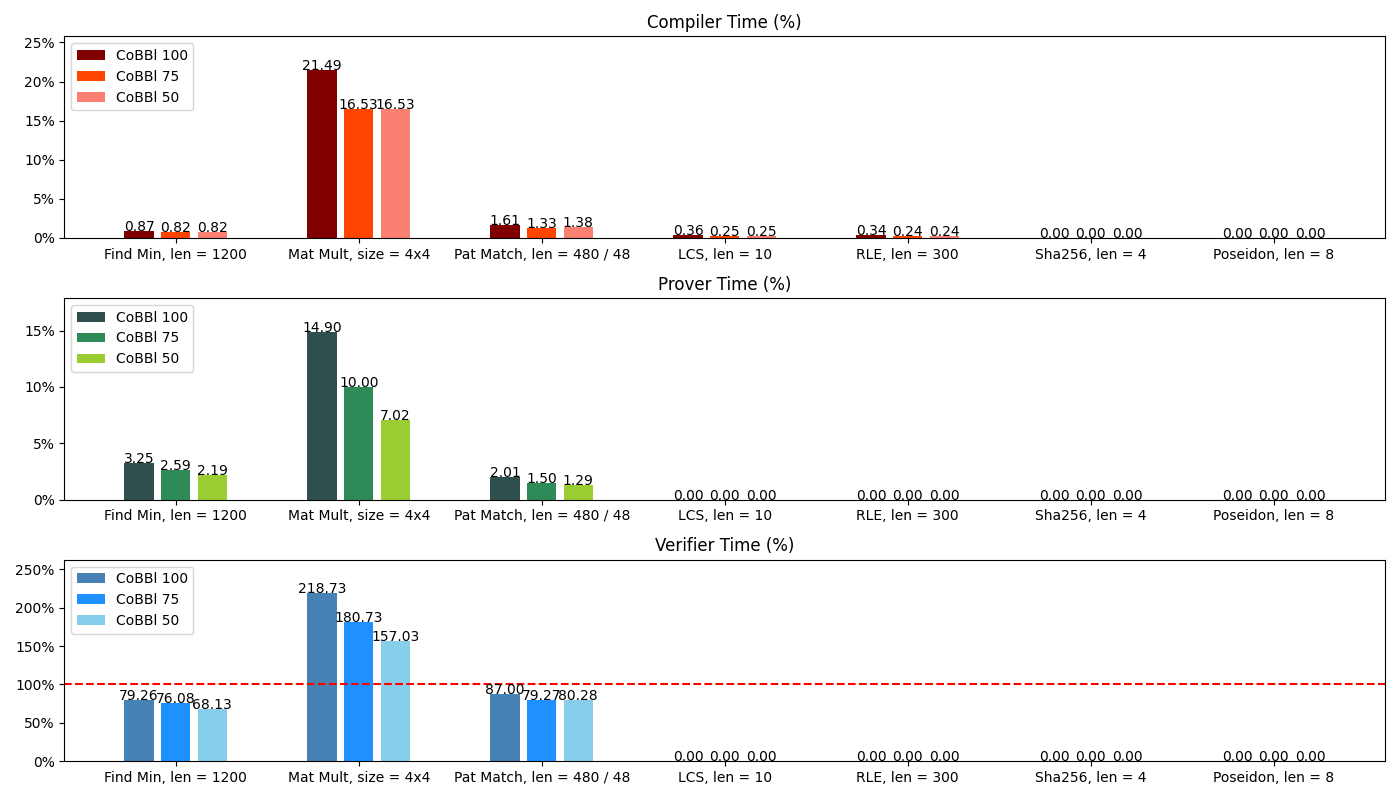
\includegraphics[width=\textwidth]{graph/fig_eval_circ.png}
  \caption{Runtime comparison between \CoBBl~and CirC.}
  \label{fig:performance_dt}
\end{figure*}
\begin{figure*}[htbp]
  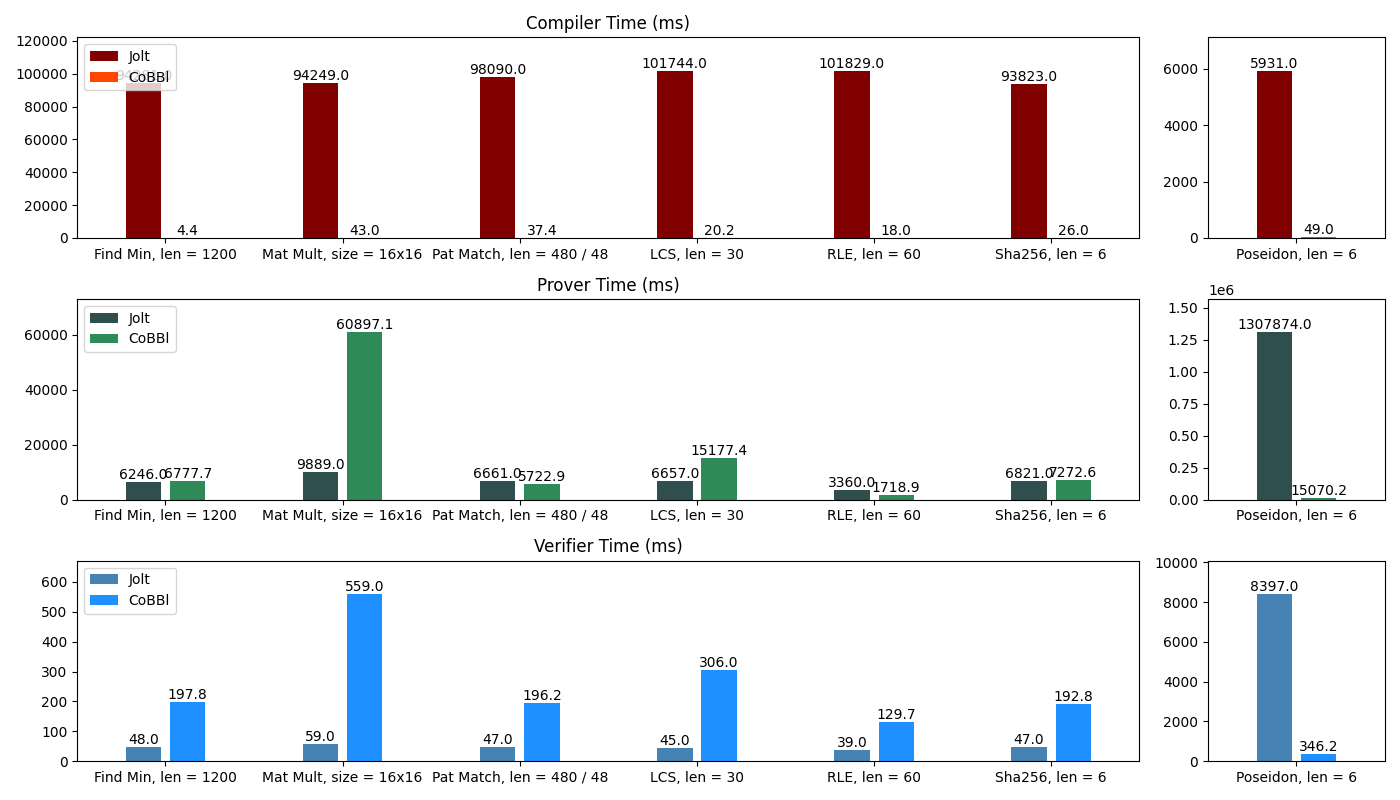
\includegraphics[width=\textwidth]{graph/fig_eval_jolt.png}
  \caption{Runtime comparison between \CoBBl~and Jolt.}
  \label{fig:performance_vm}
\end{figure*}
\begin{figure*}[htbp]
  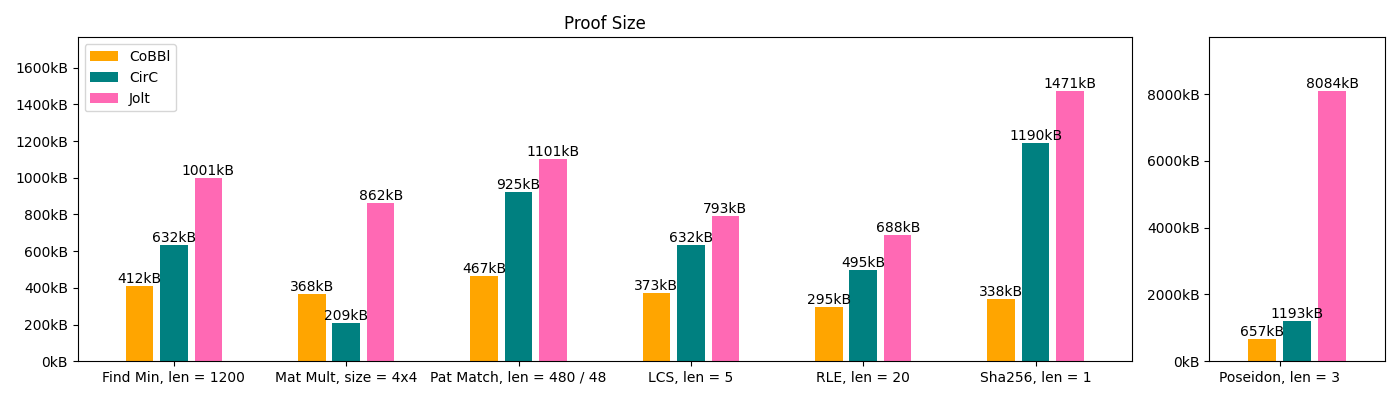
\includegraphics[width=\textwidth]{graph/fig_eval_proof_size.png}
  \caption{Proof size comparison between \CoBBl, CirC, and Jolt.}
  \label{fig:proof_size}
\end{figure*}

We present the performance comparison between \CoBBl~and CirC in figure \ref{fig:performance_dt}. \red{[XXX: Fix overlap on graph]} For each benchmark, we measure the compiler, prover, and verifier time of \CoBBl~as speedups from CirC across three input scenarios.\footnote{For matrix multiplication, we only modify the number of rows of the second matrix.} For CirC to complete more complex benchmarks, we allow polynomial commitment in both \CoBBl~and CirC to be performed in multicore. Since polynomial commitment takes up a higher percentage of CirC's computation than \CoBBl, such a setup yields more advantage towards CirC.

The results demonstrate that \CoBBl~outperforms CirC in all runtime categories across all benchmarks. \red{[XXX: Intend to increase matrix size for Mat Mult.]} In particular, \CoBBl~achieves up to 100x compiler speed up and up to 1000x prover speedup. These results closely match with our expectation: the small constraint size of \CoBBl~benefits mainly the compiler and the instance commitment phase of the prover.

We demonstrate the performance comparison between \CoBBl~and Jolt in figure \ref{fig:performance_vm}. For each benchmark, we record compiler, prover, and verifier runtime on \emph{a single CPU core}. \red{[XXX: Numbers for Poseidon are not updated.]} The results show that \CoBBl~exceeds Jolt by 3 orders of magnitude in compiler time, and for most of the benchmarks operating on 32-bit registers, is on par or better in terms of prover time. \red{[XXX: That compiler time number is embarrassing, should we even mention it?]}~\red{[XXX: How to discuss the outliers?]} For, Poseidon, a benchmark that uses primarily field operations, \CoBBl~vastly outperforms Jolt on prover time, as field operations are not present in Jolt's instruction set and require emulation using integers. We note that while Jolt's verifier is more efficient than \CoBBl~, neither incur a runtime over 600ms across any 32-bit benchmarks. Such discrepancy is seldomly taken into consideration in real-life deployment. \red{[XXX: Will there be a chance to address this earlier?]}~\red{[XXX: Will talk about verifier time once Jolt result for Poseidon is updated.]}

We present side-by-side comparison of proof size in figure \ref{fig:proof_size} and demonstrate that \CoBBl~emits smaller proofs than the two baselines across all benchmarks. \red{[XXX: Again, pending update on Mat Mult and Poseidon.]} We further comment that \CoBBl~is the only system amongst the three that does not require a static upper bound on number of witnesses. 

\subsubsection{Examining \CoBBl's improvements in detail}
\begin{figure*}[htbp]
  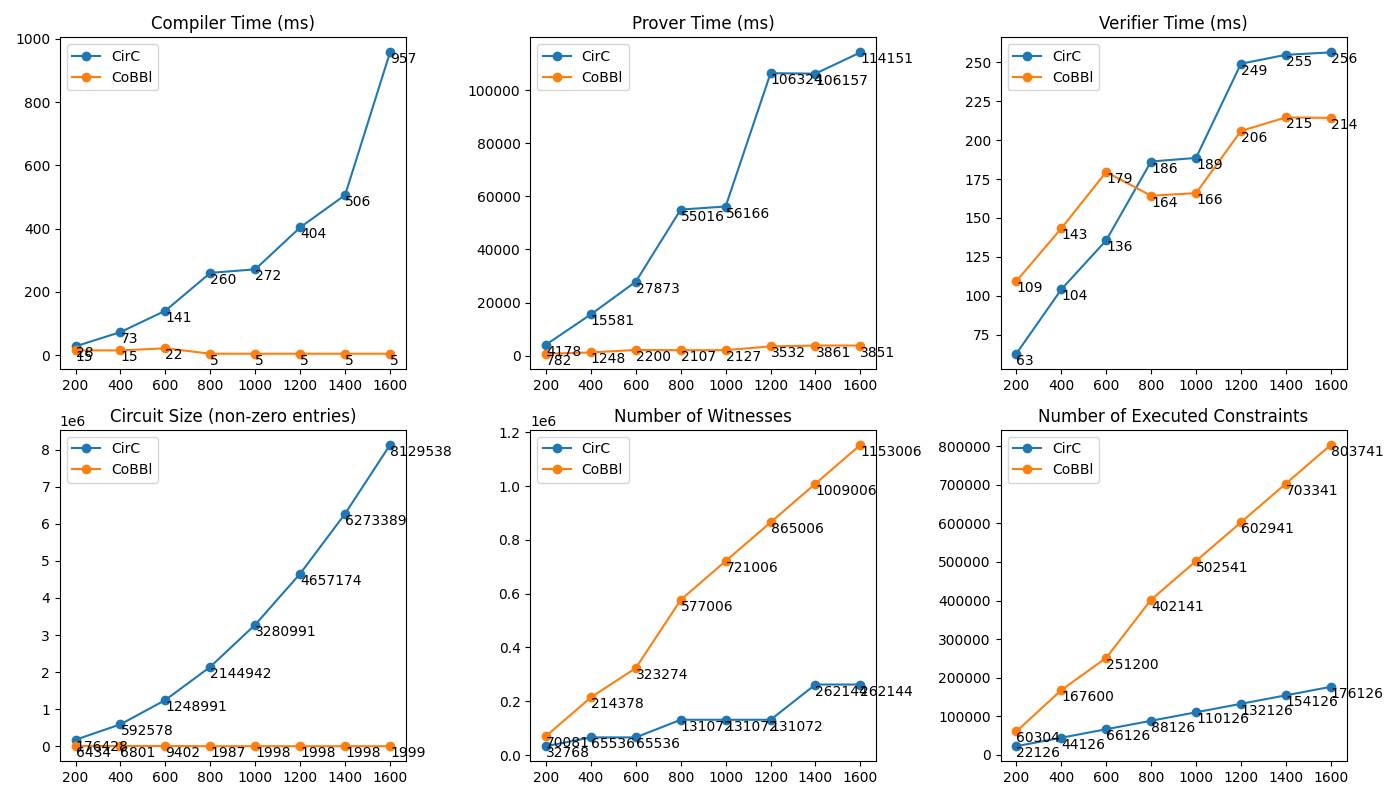
\includegraphics[width=\textwidth]{graph/fig_eval_find_min.png}
  \caption{Time and space costs for \CoBBl~and CirC on the Find Min benchmark with regarding to array length. \textbf{Circuit size} refers to the total size of the circuit emitted by the compiler. \textbf{Number of witnesses} marks the total witness size supplied by the prover. \textbf{Number of executed constraints} indicates the total amount of parallel constraints checked by the proof.}
  \label{fig:tradeoff}
\end{figure*}

To answer question \ref{q:tradeoff}, we present a detailed analysis of the Find Min benchmark in figure \ref{fig:tradeoff}. We conduct the experiment by linearly scaling the length of the array from 200 to 1600 while recording runtime and proof size across \CoBBl~and CirC.

The results demonstrate that while \CoBBl~incurs a constant factor overhead on number of witnesses and parallel constraints due to the additional program states introduced, it in turn avoids generating and committing to a circuit that expands quadratic to the size of the array. The tradeoff reflects on runtime: \CoBBl~maintains a constant compile time and linear prover time, asymptotically faster than the quadratic scaling of CirC. For verifier time, the initial constant factor in witness and parallel constraint size slows down the \CoBBl~verifier, but as array size grows and opening of the circuit commitment dominates the cost of the CirC verifier, \CoBBl~gradually outcompetes CirC on verifier time. We conclude this special benchmark by remarking that similar patterns are observed across all benchmarks during testing.